%% analyse.tex
%% $Id: analyse.tex 28 2007-01-18 16:31:32Z bless $

\chapter{Analyse}
\label{ch:Analyse}
%% ==============================

Nach der Klarstellung der grundlegenden Begrifflichkeiten im vorhergehenden Kapitel
sollen nun die Anforderungen und Limitationen der Studie festgestellt werden, die den
Zusammenhang zwischen der Nutzung von Social Media, Instant Messaging und der Geselligkeit
von Nutzern untersuchen soll. 
Dazu werden auch bereits existierende Lösungsansätze betrachtet. 

%% ==============================
\section{Anforderungen}
%% ==============================
\label{ch:Analyse:sec:Anforderungen}

%Anforderungen und Randbedingungen\index{Randbedingungen} \ldots

Für die Untersuchung des Zusammenhanges werden zwei Datensätze benötigt.
Zum einen muss die Geselligkeit der Probandin quantitativ festgehalten werden. 
Dem gegenüberstehend wird ein Datensatz, der Informationen über das Nutzungsverhalten ebenjener Probandin enthält, benötigt.
\par

\subsection{Geselligkeit}

Der Duden definiert Geselligkeit als Ungezwungenheit beim Umgang beziehungsweise dem Verkehr mit anderen Menschen und der Gesellschaft \cite{dudengesell}.
Ein solch abstraktes Konzept kann für verschiedene Menschen sehr verschiedene Formen annehmen.
Trotzdem muss für die wissenschaftliche Auseinandersetzung mit dem Thema dieses Konzept quantifiziert betrachtet werden.
Eine valides Modell dieses Problems muss durch ein standardisiertes Verfahren einen im Optimalfall numerischen Wert für diese Ungezwungenheit liefern. 
\par

Ein solches Modell, das zum Beispiel auf auch im Paper "`Who’s Who with Big-Five: Analyzing and Classifying Personality Traits with Smartphones"'\cite{chittaranjan2011s} genutzt wird, ist das Big Five Modell.
Dort ist Geselligkeit eine Unterfacette der Extraversion.
Eine oft genutzte Option um in diesem Modell numerische Werte für die verschieden Facetten und Unterfacetten zu erschließen ist eine Familie von Selbstbeurteilungsfragenbogen,
die zum Beispiel auch in T. Correa's "`Who interacts on the Web?: The intersection of users’ personality and social media use"' \cite{butt2008personality} genutzt wird.
Zu dieser Familie gehören unter anderem der ursprünglichen NEO-Inventory-  von 1978, der NEO-Personality Inventory- (NEO-PI) von 1985 und der NEO-Five Factor Inventory-Fragenbogen (NEO-FFI).
Im Rahmen dieser Arbeit wird der auf dem NEO-PI basierende überarbeitete NEO-Personality Inventory-Revised-Fragebogen (NEO-PI-R) in der Version von 2003 benutzt\cite{neopir2003}
um der Extraversion und der Geselligkeit der einzelnen Testprobandinnen einen numerischen Wert zuzuordnen.

Die Entscheidung für den NEO-PI-R liegt nahe: 
Er ist gemeinsam mit dem NEO-FFI der aktuellste Fragebogen dieser Familie und liefert mit seinen insgesamt 241 Fragen, davon zumindest 48 Fragen auf Extraversion bezogen,
einen nuancierterer Blick auf die Persönlichkeit der durchführenden Person als der NEO-FFI, der insgesamt nur 60 Fragen hat und dementsprechend nur mit 12 Fragen zur Extraversion aufwartet.



\subsection{Nutzungsdaten}

Von besonderer Relevanz für das Sammeln der Nutzungsdaten ist es festzulegen welche Daten zur Verfügung stehen, welche relevant sind und welche potenziell trotzdem nicht gesammelt werden sollten.
Für diese Arbeit werden keine Nutzerdaten von physische Sensoren in Betracht gezogen, sondern nur die Interaktion mit dem Smartphone als Kommunikationsgerät.
Zu diesem Zweck interagiert die Applikation mit Schnittstellen des Android Betriebssystems.
Dies vermeidet das potenzielle Problem von unterschiedlicher Hardware und sorgt dafür, dass die Nutzungsdaten von allen Testprobanden vergleichbar bleiben.
Zudem vermeidet dies übermäßige Mehrbelastung der Akkuleistung der Smartphones, auf denen die Applikation installiert wird.
Allgemein ist es wünschenswert die Belastung der Ressourcen auf den Zielgeräten so gering wie möglich zu halten.
\par

Eine der stärksten Limitation für die Daten, die die Applikation sammeln kann, kommt von der persönlichen Natur der zu betrachtenden Daten.
Zum einen begrenzt das Android Betriebssystem selbst die Informationen zu denen eine Applikation, selbst eine die vom Nutzer mit potenziell jeder Berechtigung ausgestattet wurde, Zugang hat.
Dies geschieht aus Datenschutzgründen, da manche Applikationen im Play Store mehr Berechtigungen einfordern als sie für ihre Funktionstüchtigkeit benötigen würden.
Zum anderen sind die Kommunikationsapplikationen, die die Testprobandin nutzt von unabhängigen Drittentwicklern entworfen worden.
Einige Wenige von diesen stellen in ganz speziellen Fällen, zum Beispiel Twitter\cite{twitterapi}, zwar eine API zur Verfügung, die meisten hüten ihre Daten aber.
Folglich können nur Daten gesammelt werden, die entweder frei zugänglich sind, oder solche, zu denen die Nutzerin Applikationen Zugriff erlauben kann.
Beispiele hierfür sind zum Beispiel die Call logs in denen Android, für alle Apps mit der Berechtigung \textbf{android.permission.READ\_CALL\_LOG}, die vergangenen Anrufe abspeichert.
\par

In diesem Kontext ist das Android API Ziellevel der Applikation von großer Bedeutung.
Wie bei Smartphone Betriebssystemen üblich wird das Android Betriebssystem konstant weiterentwickelt und neue Versionen davon werden ausgeliefert.
Potenzielle Änderungen an Systemschnittstellen werden dabei durch die verschiedenen API Levels dokumentiert, auf die sich installierte Applikationen berufen können.
Die aktuellste Version von Android ist Android 6.0, oder auch Android Marshmallow.
Diese wird repräsentiert durch das API Level 23.
Da nicht alle Geräte die steigenden Anforderungen aktuellerer Android Versionen erfüllen, 
und manche Nutzer neu herauskommende Updates selbst dann nicht installieren, wenn ihr Gerät sie unterstützt, 
%sei es auf Grund von Faulheit, Unwissenheit oder Bequemlichkeit,
sind auf vielen Smartphones ältere Android Versionen vertreten.
Eine Übersicht über die Verteilung der Android Versionen ist in Diagramm \ref{fig:androidplatformdistr} zu sehen.
Mit 36.1\% ist Android 5, beziehungsweise Android Lollipop die am weitesten verbreitetste Version,
gefolgt von Android 4.4 (Kitkat) mit 34.3\% und Android 4.0-4.3 (Jellybean) mit 22.3\%\cite{androiddistr}.
Für die Entwicklung der Applikation wird Android API level 21, entspricht Android 5.0, als Ziellevel bestimmt, da es einige relevante Schnittstellen hinzufügt die bei niedrigeren Leveln noch nicht existieren, aber auch eine breit genuge Userbasis hat, um ausreichend viele Probandinnen zu finden.


\begin{figure}[h]
    \centering
    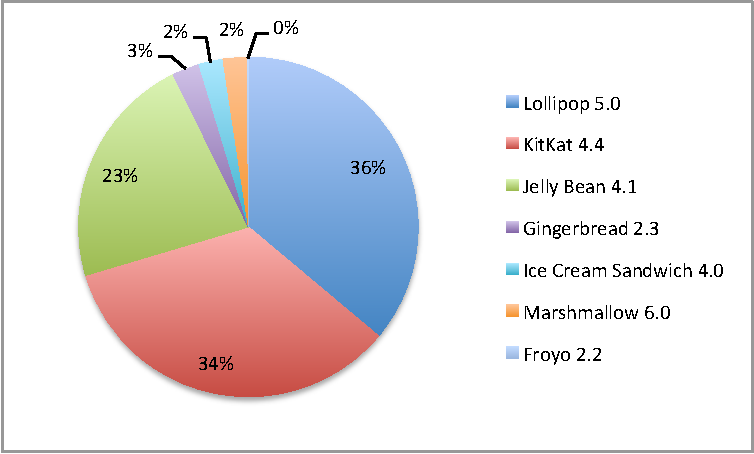
\includegraphics{images/chart.pdf}
    \caption{Android Platform Distribution\cite{androiddistr}}
    \label{fig:androidplatformdistr}
\end{figure}

Auch die Sensibilitäten potenzieller Testprobandinnen müssen in Betracht gezogen werden:
Während die Anzahl an Anrufen in den vergangenen 14 Tagen von vielen als unkritisch betrachtet werden würde, so gibt es sicher eine Menge Menschen, 
die eine Liste von Telefongesprächen inklusive Zeitpunkt und Rufnummer des Partners als zu tiefen Eingriff in ihre Privatsphäre wahrnehmen würden.
Ziel muss es hier sein bezüglich der Geselligkeit aussagekräftige Datenpunkte zu wählen, 
die aber dennoch nicht das grundlegende Bedürfnis nach Privatsphäre der Probandinnen verletzt.


\subsection{Datenschutz}

Die Daten mit denen im Rahmen dieser Studie gearbeitet werden sind sehr sensibler Natur.
Dementsprechend muss sicher gestellt werden, dass sowohl die Anonymität der einzelnen Probandinnen gewahrt bleibt,
als auch, dass die Daten nicht den Rahmen der Studie verlassen.
Dazu werden die erhobenen Daten pseudonymisiert, das heißt zur Idenfikation der Zugehörigkeit von Fragebogen und erhobenen Daten wird nicht der Name der Versuchsteilnehmerin genutzt, sondern ein frei gewähltes Pseudonym.
Außerdem werden keinerlei persönlichkeitsbezogene Daten im Klartext gespeichert.
Weder Telefonnummern, noch Absender oder Nachrichteninhalte werden in Klartext geloggt.
Stattdessen werden die relevanten Features der Daten in anderer Form abgespeichert:
Unter anderem Anzahl verschiedener Telefonnummern, durch Hashen unkenntlich gemachte Nachrichtenabsender und Ersetzen der Nachrichtentexte durch die Anzahl der Zeichen in der Nachricht.
Dennoch wird, wie bei allen Studien dieser Art, die am TECO durchgeführt werden,
eine unterschriebene Einwilligungserklärung seitens der Probandin benötigt.
In dieser wird das Einverständnis der Probandin bezüglich der Aufzeichnung, Speicherung und Verarbeitung ihrer Daten zugesichert.
\ignore{siehe Anhang, adde anhang?}
\par



%% ==============================
\section{Existierende Lösungsansätze}
%% ==============================
\label{ch:Analyse:sec:RelatedWork}

Die Auswahl der zu untersuchenden Smartphonedaten haben verschiedene bisher existierende Arbeiten unterschiedlich gelöst.
Ebenso gibt es in den Studien im Feld verschiedene Ansätze wie die Persönlichkeit von Testprobandinnen in vergleichbare Werte zu fassen ist.

\subsection{Persönlichkeit}

In der Familie der NEO Fragebögen gibt es verschiede Versionen und Iterationen, die für verschiedene Situationen benutzt werden können.
Neben dem Urspünglichen NEO - Personality Inventory von 1978 sind heutzutage vorallem der NEO - PI - R und der NEO - FFI im Einsatz.
Von den fünft im Kapitel \ref{ch:Grundlagen:sec:RelatedWork} vorgestellten Arbeiten benutzen drei den NEO-FFI Fragenbogen. 
Dieser mit seinen 60 Fragen gering im Umfang, nicht zu komplex und benötigt nicht zu viel Zeit um ausgefüllt zu werden.

\par
TODO: Aussschmücken, vll noch was zum Selbstwertgefühl inventar?

\par
Im Rahmen dieser Arbeit eignet sich der NEO-PI-R besser als der in den verwandten Arbeiten häufig genutzte NEO-FFI, 
da um die geringere Menge an Probandinnen auszugleichen eine detailliertere Betrachung wünschenswert ist und 
er zudem nicht nur Extraversion allgemein betrachtet sondern auch dessen Unterfacetten, unter denen sich die Geselligkeit befindet.

\subsection{Smartphone Daten}

\ignore{se}
Anstatt der weithin gängigen Praxis, die unter anderem auch in den Arbeiten von Butt \cite{butt2008personality} und Lane \cite{lane2011impact}
eingesetzt wird, sich auf Selbsteinschätzungen der Probandinnen zu verlassen sollen aussagekräftige Daten direkt vom Smartphone gesammelt werden, 
wie es Chittaranjan \cite{chittaranjan2011s} und Wang \cite{wang2014istudentlife} in ihren Arbeiten tun.
\par
Die von Chattaranjan gesammelten Datenpunkte sind zumindest für SMS und Anrufe sinnvoll und können größtenteils übernommen werden.
Der Sprung von Nokias Symbian Betriebssystem zu Googles Android ist hier unproblematisch da beide Applikationen die Möglichkeit geben können
vergangene Anrufe und SMS zu betrachten.
Kritischer zu betrachten sind die bezüglich Applikationen gesammelten Daten.
Die Studie betrachtet ausschließlich Anzahl der Nutzungen von Applikationen der folgenden Kategorien:
Office, Internet, Video/Audio/Musik, Maps, Mail, Youtube, Calender, Camera, Chat, SMS, Games.
Weder die Nutzungsdauer, noch Interaktionen durch die Applikationen werden betrachtet. 
Dadurch ist die Studie, obwohl sie nur 5 Jahre in der Vergangenheit liegt, zumindest bezüglich der Applikationsnutzung nicht mehr relevant.
Wie die Statistik \ref{smsvswhatsapp} nahelegt vollzieht sich in den letzten Jahren eine Verschiebung der Kommunikationsgewohnheiten hin zu Messengern und weg von konventionelleren Kommunikationswegen wie SMS.
Dementsprechend soll im Rahmen dieser Studie ein größerer Fokus auf die Applikationen gelegt werden.
\par
In dieser Arbeit ist es leider nicht möglich so weit zu gehen wie Wang.
In seiner Arbeit werden Ressourcen benutzt, wie die Echtzeitanalyse der mitgeschnittenen Tonspuren und die akademischen Ergebnisse der Probandinnen, die weit jenseits der Möglichkeiten einer Bachelorarbeit liegen.
Außerdem ist das mehrfache EMA ausfüllen pro Tag ein sehr invasiv in den Alltag der Probanden, was potenziell auch deren Verhalten beeinflusst.
Im Rahmen dieser Arbeit soll so wenig wie möglich in den Alltag der einzelnen Probandin eingegriffen werden, sodass diese so wenig wie möglich von der Studie beeinflusst wird.


\begin{figure}[h]
    \centering
    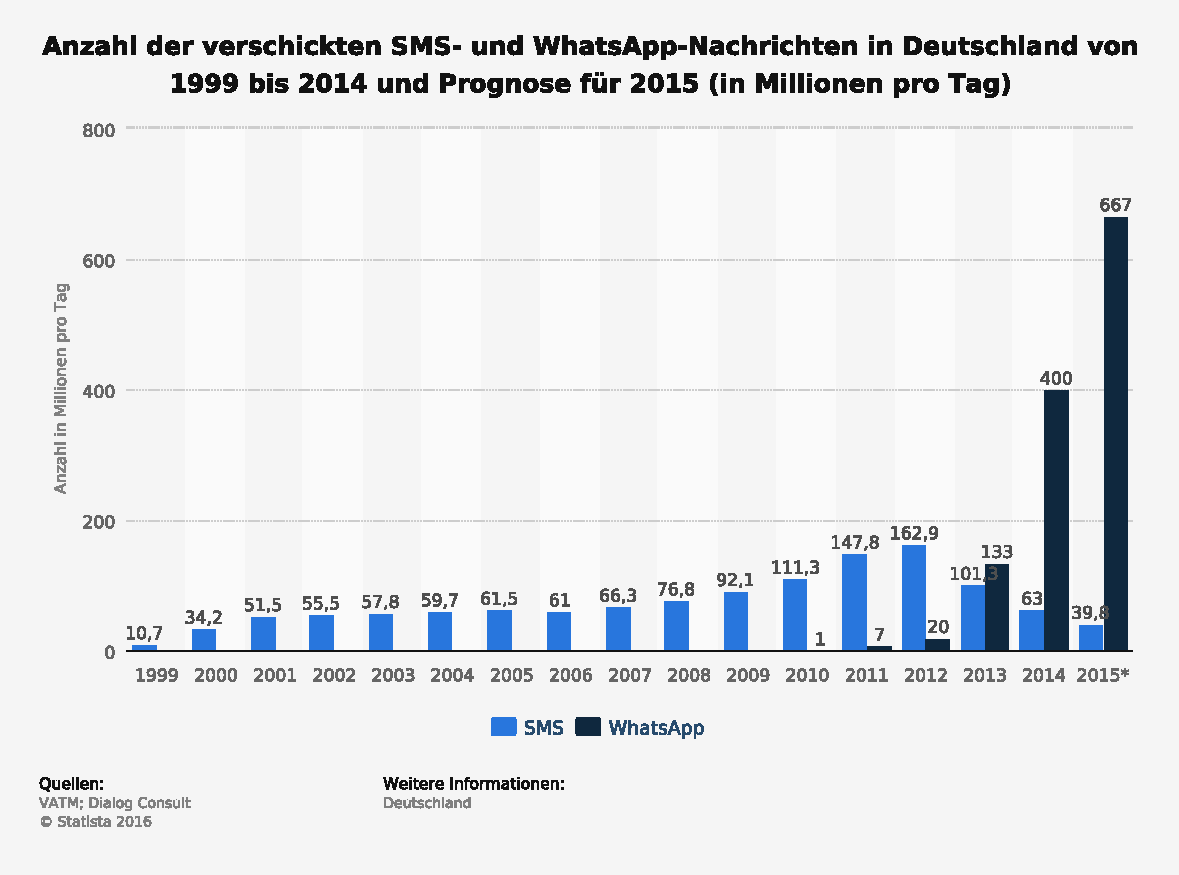
\includegraphics[width=\textwidth]{images/statistic_id3624_anzahl-gesendeter-sms-nachrichten-pro-tag-in-deutschland-bis-2015}
    \caption{Vergleich versendete SMS und Whatsapp-Nachrichten pro Jahr\cite{whatsappVergleichSMS}}
    \label{smsvswhatsapp}
\end{figure}


%% ==============================
\section{Zusammenfassung}
%% ==============================
\label{ch:Analyse:sec:zusammenfassung}

Für diese Arbeit sind die Wahl eines sinnvollen Modells für die Messung der Geselligkeit eines Menschen 
und die Auswahl von relevanten und verfügbaren Daten, die mittels der Android Applikation gesammelt werden sollen, von zentraler Bedeutung.
Zur Messung der Geselligkeit wird der NEO-PI-R Fragebogen eingesetzt werden.
Die Android Applikation wird Daten bezüglich des Anruf und SMS Verhaltens der Probandinnen sammeln,
sowie eine Liste an empfangenen Notifications anlegen und die UsageStat Schnittstelle des Android Betriebssystems nutzen.
Für die Applikation ist außerdem wichtig, dass sie so leichtgewichtig wie möglich ist, 
sowohl was die Bedienung durch die Probandinnen angeht, als auch den Stromverbrauch und die Belastung auf Speicher und Prozessor.
Alle erhobenen Daten müssen im Kontext von Datenschutz und Schutz der Privatsphäre betrachtet und überdacht werden, weshalb die persönlichkeitsbezogenen Daten aus den Notifications entweder gehasht oder nur abstrahiert als numerischen Wert der Länge des Textes gespeichert werden.
Anrufe und SMS werden nur in bereits konzentrierter Form gespeichert und nicht nicht als Liste von Ereignissen.

%%% Local Variables: 
%%% mode: latex
%%% TeX-master: "diplarb"
%%% End: 
